\documentclass[conference]{IEEEtran}
\IEEEoverridecommandlockouts

\usepackage{cite}
\usepackage{amsmath,amssymb,amsfonts}
\usepackage{algorithmic}
\usepackage{algorithm}
\usepackage{graphicx}
\usepackage{textcomp}
\usepackage{xcolor}
\usepackage{hyperref}
\usepackage{listings}
\usepackage{booktabs}
\usepackage{multirow}
\usepackage{tabularx}
\usepackage{tikz}
\usepackage{pgfplots}
\pgfplotsset{compat=1.18}
\usetikzlibrary{shapes.geometric, arrows.meta, positioning, fit, backgrounds, shadows}

\hypersetup{
  colorlinks=true,
  linkcolor=blue,
  citecolor=blue,
  urlcolor=blue
}

\lstset{
  basicstyle=\ttfamily\footnotesize,
  backgroundcolor=\color{gray!10},
  frame=single,
  framerule=0.4pt,
  rulecolor=\color{gray!50},
  breaklines=true,
  captionpos=b,
  numbers=left,
  numberstyle=\tiny\color{gray},
  numbersep=5pt,
  tabsize=2,
  showstringspaces=false,
  keywordstyle=\color{blue!70}\bfseries,
  commentstyle=\color{green!50!black},
  stringstyle=\color{red!60},
  language=Python
}

\def\BibTeX{{\rm B\kern-.05em{\sc i\kern-.025em b}\kern-.08em
    T\kern-.1667em\lower.7ex\hbox{E}\kern-.125emX}}

% ─────────────────────────────────────────────────────────────────────────────
\begin{document}

\title{Lumina: A Distributed Split Inference System\\
{\large An Enterprise Distributed Systems Architecture for Cross-Node Neural Network Layer Partitioning}}

\author{
  \IEEEauthorblockN{Ekant Kapgate, Hei Lam, Pranav Jitendra Trivedi, Shefali Saini}
  \IEEEauthorblockA{
    \textit{Department of Computer Engineering, San Jose State University}\\
    San Jose, CA, USA\\
  }
}

\maketitle

% ─────────────────────────────────────────────────────────────────────────────
\begin{abstract}
Large language models demand GPU memory that exceeds the capacity of individual
consumer-grade machines. Lumina addresses this constraint by implementing a
\emph{split inference} architecture that partitions a transformer model's layers
across two physically separate compute nodes. A stateful Tracker service
dynamically recalculates the optimal split point at runtime based on each
node's available VRAM, communicating the assignment via a versioned REST API.
Intermediate hidden-state tensors are serialized using PyTorch's native binary
format, base64-encoded, and transmitted over standard HTTP, enabling deployment
on commodity hardware without specialized interconnects. The system is
containerized with Docker, provisioned via Terraform, and deployed across three
AWS EC2 instances. From an enterprise distributed systems perspective, Lumina
demonstrates microservices decomposition, service self-registration, dynamic
configuration, fault-tolerant fallback, infrastructure as code, and a full
observability pipeline. This paper presents the system architecture,
implementation details, deployment topology, and a discussion of enterprise
patterns including CAP theorem implications, service mesh considerations, and
production scaling pathways.
\end{abstract}

\begin{IEEEkeywords}
split inference, distributed systems, microservices, transformer partitioning,
service discovery, dynamic configuration, AWS, Terraform, FastAPI, PyTorch
\end{IEEEkeywords}

% ─────────────────────────────────────────────────────────────────────────────
\section{Introduction}

The rapid growth of large language models (LLMs) has created a significant
resource barrier for practitioners operating outside hyperscale cloud
environments. Qwen2.5-1.5B-Instruct~\cite{qwen2025}, the model used in this work,
has 28 transformer layers and 1.5 billion parameters. Even at this relatively
modest scale, fully loading the model on a single CPU machine requires several
gigabytes of RAM—a constraint that worsens as models grow. As models scale to
tens of billions of parameters, a single consumer GPU is entirely insufficient
to host the complete model graph.

\emph{Split inference}---the practice of partitioning a neural network's
computational graph across multiple devices---has emerged as a practical
response to this constraint~\cite{kang2017neurosurgeon}. Rather than requiring
a monolithic accelerator, split inference allows organizations to aggregate the
capacity of multiple commodity machines, each hosting a shard of the model.

Lumina implements a three-node split inference pipeline. Node~A (head) runs
layers 0--8, Node~B (mid) runs layers 9--18, and Node~C (tail) runs layers
19--27 plus the final normalization and language model head. The system is
designed around enterprise distributed systems principles: services are
independently deployable, communicate via versioned REST APIs, self-register
with a coordination service, and expose health and observability endpoints.
The project serves as a proof-of-concept for distributed LLM inference
deployable on commodity hardware without specialized networking or GPUs.

The key contributions of this work are:

\begin{itemize}
  \item A dynamic layer-partitioning algorithm that adapts split boundaries at
        inference time based on node VRAM ratios.
  \item A stateful coordination service (Tracker) implementing service
        discovery, heartbeat-based liveness, and versioned assignment
        distribution.
  \item A tensor transport protocol using PyTorch serialization over
        base64-encoded HTTP, requiring no custom RPC infrastructure.
  \item A complete Infrastructure-as-Code deployment (Terraform + Docker)
        targeting AWS EC2 and AWS Fargate.
  \item A memory-aware model loading strategy that reads only each node's
        assigned layer slice directly from safetensors shards, using a
        \texttt{meta}-device skeleton so unused weights are never materialized.
  \item An observability frontend providing real-time cluster state, generation
        chat, request trace visualization, and a client-side structured log
        viewer backed by \texttt{localStorage}.
\end{itemize}

% ─────────────────────────────────────────────────────────────────────────────
\section{Related Work}

\subsection{Model Parallelism}

Model parallelism, or tensor parallelism, is well established in the deep
learning literature. Megatron-LM~\cite{shoeybi2019megatron} demonstrated that
transformer layers can be partitioned across GPUs with minimal communication
overhead using tensor-level splits. PipeSwitch~\cite{bai2020pipeswitch}
introduced pipeline parallelism for multi-tenant GPU servers. Lumina adopts a
simpler pipeline split---a single cut point between layers---prioritizing
deployability over throughput.

\subsection{Edge Inference Partitioning}

Neurosurgeon~\cite{kang2017neurosurgeon} and JALAD~\cite{li2018jalad} explored
splitting deep neural networks between edge devices and cloud servers to reduce
end-to-end latency. These works motivate the dynamic split assignment in
Lumina: the optimal cut point depends on available compute and network
conditions, both of which vary at runtime. Lumina's Tracker implements a
simplified version of this dynamic assignment using VRAM as the primary signal.

\subsection{Microservices for ML Systems}

The application of microservices patterns to machine learning inference
pipelines has gained traction through systems such as Clipper~\cite{crankshaw2017clipper}
and KServe~\cite{kserve2023}. These systems emphasize model versioning, A/B
testing, and SLA guarantees. Lumina applies the same decomposition
principles---separating compute, coordination, and presentation concerns into
independent services---but targets the novel domain of split inference rather
than ensemble serving.

\subsection{Tensor Serialization}

Prior work on distributed tensor computation typically employs
NCCL~\cite{jeaugey2017nccl} or gRPC with Protocol Buffers for inter-node
communication. Lumina adopts a simpler approach: PyTorch's \texttt{torch.save()}
API produces a binary blob that is base64-encoded and embedded in a JSON HTTP
body. While less efficient than binary RPC, this approach requires no custom
serialization infrastructure and operates over standard HTTP/1.1.

% ─────────────────────────────────────────────────────────────────────────────
\section{System Architecture}

Lumina comprises five independently deployed components: Node~A (head),
Node~B (mid), Node~C (tail), the Tracker coordination service, and a React
frontend dashboard. Figure~\ref{fig:arch} illustrates the high-level system
architecture. The model (Qwen2.5-1.5B-Instruct, 28 layers) is partitioned
across the three inference nodes with a default split of 9/10/9 layers.

% ── System Architecture Diagram ──────────────────────────────────────────────
\begin{figure*}[t]
\centering
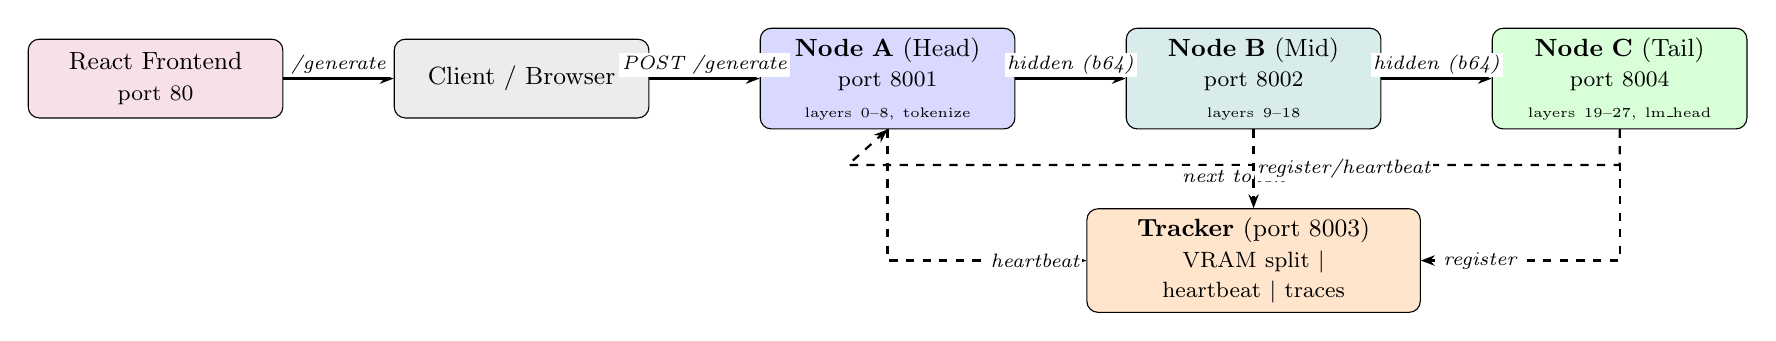
\begin{tikzpicture}[
  node distance=0.5cm and 1.4cm,
  box/.style={rectangle, rounded corners=4pt, draw, text width=3.0cm,
              minimum height=1.0cm, align=center, font=\small},
  wide/.style={rectangle, rounded corners=4pt, draw, text width=4.0cm,
               minimum height=1.0cm, align=center, font=\small},
  arrow/.style={-{Stealth[length=5pt]}, thick},
  darrow/.style={-{Stealth[length=5pt]}, thick, dashed},
  lbl/.style={font=\scriptsize\itshape, fill=white, inner sep=1pt}
]

% Top row: Frontend  Client
\node[box, fill=purple!12] (fe)     {React Frontend\\{\footnotesize port 80}};
\node[box, fill=gray!15,   right=of fe] (client) {Client / Browser};

% Inference chain (horizontal)
\node[box, fill=blue!15,   right=of client] (nodea)
  {\textbf{Node A} (Head)\\{\footnotesize port 8001}\\
   {\tiny layers 0--8, tokenize}};
\node[box, fill=teal!15,   right=of nodea]  (nodeb)
  {\textbf{Node B} (Mid)\\{\footnotesize port 8002}\\
   {\tiny layers 9--18}};
\node[box, fill=green!15,  right=of nodeb]  (nodec)
  {\textbf{Node C} (Tail)\\{\footnotesize port 8004}\\
   {\tiny layers 19--27, lm\_head}};

% Tracker below the chain
\node[wide, fill=orange!20, below=1.0cm of nodeb] (tracker)
  {\textbf{Tracker} (port 8003)\\
   {\footnotesize VRAM split \textbar{} heartbeat \textbar{} traces}};

% Data flow arrows
\draw[arrow] (fe)     -- node[lbl, above]{/generate} (client);
\draw[arrow] (client) -- node[lbl, above]{POST /generate} (nodea);
\draw[arrow] (nodea)  -- node[lbl, above]{\scriptsize hidden (b64)} (nodeb);
\draw[arrow] (nodeb)  -- node[lbl, above]{\scriptsize hidden (b64)} (nodec);

% Return path: next token back to Node A (below the chain)
\draw[darrow] (nodec.south) -- ++(0,-0.45)
              -- node[lbl, below]{next token} ++(-9.8,0)
              -- (nodea.south);

% Heartbeat / register arrows to Tracker
\draw[darrow] (nodea.south) |- node[lbl, right, near end]{heartbeat} (tracker.west);
\draw[darrow] (nodeb.south) -- node[lbl, right]{register/heartbeat} (tracker.north);
\draw[darrow] (nodec.south) |- node[lbl, left, near end]{register} (tracker.east);

\end{tikzpicture}
\caption{Lumina 3-node split inference architecture. The inference pipeline flows
left to right: Node~A tokenizes the prompt and runs layers 0--8, Node~B relays
layers 9--18, and Node~C runs layers 19--27 and returns the next token.
All nodes send periodic heartbeats to the Tracker, which maintains the dynamic
split assignment. Solid arrows: data flow; dashed arrows: control/registration flow.}
\label{fig:arch}
\end{figure*}

\subsection{Node A --- Head Service}

Node~A serves as the system's public inference endpoint. On receipt of a
\texttt{POST /generate} request, it tokenizes the input prompt and initiates
an autoregressive generation loop. For each token position it runs the token
embedding, positional embedding, and transformer layers 0--8 of the
Qwen2.5-1.5B model. The resulting hidden-state tensor is base64-encoded and
forwarded to Node~B via \texttt{POST /forward\_mid}.

Node~A also consults the Tracker's \texttt{/assignment} endpoint at the start
of each generate call to refresh the current split boundaries
(\texttt{split\_layer\_a}, \texttt{split\_layer\_b}). A background daemon
thread heartbeats the Tracker every 20~s independently of incoming requests,
ensuring liveness is maintained even during idle periods.

\subsection{Node B --- Middle Service}

Node~B exposes \texttt{POST /forward\_mid}. It receives hidden states from
Node~A, runs transformer layers 9--18, and immediately forwards the resulting
hidden states to Node~C via \texttt{POST /forward\_tail}. Node~B maintains no
generation state; it is a pure compute relay. Like all nodes it runs a
background heartbeat thread every 20~s.

\subsection{Node C --- Tail Service}

Node~C exposes \texttt{POST /forward\_tail}. It receives hidden states from
Node~B, runs transformer layers 19--27, applies the final layer normalization
and language model head, and returns the argmax next token as a base64-encoded
tensor. All autoregressive context (token IDs, attention mask) is tracked
exclusively by Node~A; Node~C is stateless across requests.

\subsection{Tracker --- Coordination Service}

The Tracker is a stateful coordination service responsible for dynamic split
assignment. It maintains an in-memory registry of all active nodes, keyed by
\texttt{node\_id}. Each registry entry records the node's role (head or tail),
reported VRAM in gigabytes, maximum layer capacity, and the monotonic timestamp
of its last heartbeat.

The core rebalancing algorithm, shown in Algorithm~\ref{alg:rebalance},
executes on every heartbeat event.

\begin{algorithm}[htbp]
\caption{Tracker Rebalance Algorithm}
\label{alg:rebalance}
\begin{algorithmic}[1]
\STATE $head \leftarrow$ \textsc{ActiveNode}(\textit{role}=``head'')
\STATE $tail \leftarrow$ \textsc{ActiveNode}(\textit{role}=``tail'')
\IF{$head = \text{None}$ \textbf{or} $tail = \text{None}$}
  \STATE $target \leftarrow fallback\_split\_layer$
\ELSE
  \STATE $ratio \leftarrow head.vram / (head.vram + tail.vram)$
  \STATE $target \leftarrow \text{round}(ratio \times total\_layers)$
  \STATE $head\_cap \leftarrow \min(head.max\_layers,\ total\_layers - 1)$
  \STATE $tail\_min \leftarrow total\_layers - tail.max\_layers$
  \STATE $target \leftarrow \text{clamp}(target,\ tail\_min,\ head\_cap)$
\ENDIF
\IF{$target \neq current\_split\_layer$}
  \STATE $current\_split\_layer \leftarrow target$
  \STATE $version \mathrel{+}= 1$
\ENDIF
\end{algorithmic}
\end{algorithm}

A node is considered stale if its \texttt{last\_seen} timestamp exceeds
\texttt{heartbeat\_timeout\_sec} (120~s in cloud deployments, 30~s default).
The extended timeout accommodates the slow model-load startup time on CPU-only
instances. When all three active nodes are present, split boundaries are
computed proportionally to VRAM. A version counter increments on every split
change, allowing clients to detect assignment drift without maintaining local
state.

\subsection{Frontend Dashboard}

The React/Vite frontend provides five views: a \emph{Chat} page for interactive
text generation, a \emph{Health} page showing per-service status, a
\emph{Cluster} page displaying live node statistics (CPU\%, RAM usage, VRAM,
latency, active connections, and sharing topology), a \emph{Trace} page
displaying request history with per-request duration, and a \emph{Logs} page
rendering in-browser activity logs persisted to \texttt{localStorage}.

The \emph{Cluster} page was extended to show summary cards for total, active,
and inactive node counts. The polling hooks (\texttt{useNodePolling},
\texttt{useHealthPolling}) were updated to emit structured log entries via a
client-side \texttt{frontendLogger} utility, capturing event level, message,
and metadata (node count, active nodes, API error strings). Logs are capped at
150 entries in localStorage and displayed in a live-updating table that
refreshes every 2~seconds. The frontend communicates directly with Node~A and
the Tracker via Axios, with nginx serving static assets on the frontend EC2
instance.

% ─────────────────────────────────────────────────────────────────────────────
\section{Implementation Details}

\subsection{Tensor Transport Protocol}

The core technical challenge of split inference over a standard HTTP API is the
serialization of intermediate tensor state. The \texttt{tensor\_codec} module
implements a two-step encoding pipeline, shown in Listing~\ref{lst:codec}.

\begin{lstlisting}[caption={Tensor codec: PyTorch binary format over base64-encoded HTTP.}, label={lst:codec}]
def tensor_to_b64(tensor: Tensor) -> str:
    buf = BytesIO()
    torch.save(tensor.detach().cpu(), buf)
    return b64encode(buf.getvalue()).decode()

def b64_to_tensor(val: str,
                  device: torch.device) -> Tensor:
    data = b64decode(val.encode())
    return torch.load(BytesIO(data),
                      map_location=device)
\end{lstlisting}

The \texttt{TailForwardRequest} schema carries three tensors:
\texttt{token\_ids\_b64} (current input IDs), \texttt{attention\_mask\_b64},
and \texttt{hidden\_states\_b64} (the head computation output). Using
\texttt{torch.save()} rather than a raw NumPy dump preserves tensor metadata
including dtype and device mapping, enabling correct deserialization regardless
of the receiving node's hardware configuration.

\subsection{Autoregressive Generation Loop}

GPT-2 is a decoder-only model that generates text one token at a time, with
each token conditioned on all previous tokens. Lumina implements this
autoregressive loop in Node~A as shown in Listing~\ref{lst:loop}.

\begin{lstlisting}[caption={Autoregressive generation loop in Node A.}, label={lst:loop}]
for _ in range(max_new_tokens):
    hidden = run_head(ids)       # layers 0-8
    payload = MidForwardRequest(
        hidden_states_b64=encode(hidden), ...)
    # Node B runs layers 9-18, then calls Node C
    # Node C runs layers 19-27, returns next token
    resp = POST(node_b_url + "/forward_mid", payload)
    next_tok = decode(resp.generated_token_ids_b64)
    ids = cat([ids, next_tok], dim=1)
    if next_tok == eos_token:
        break
\end{lstlisting}

Each token requires two chained HTTP hops: Node~A~$\to$~Node~B~$\to$~Node~C.
Node~B acts as a relay, immediately forwarding its output to Node~C without
returning to Node~A. This keeps the critical path at two round trips per token
rather than three, while preserving the stateless relay design. For a 20-token
generation, the system performs 40 HTTP requests in total across the three
nodes.

\subsection{Service Self-Registration}

All three inference nodes (Node~A, Node~B, Node~C) register with the Tracker
on FastAPI startup via the \texttt{on\_event('startup')} hook. The registration
payload includes the node's unique identifier, role (\texttt{head},
\texttt{mid}, or \texttt{tail}), estimated VRAM, maximum layer capacity, and
total model layer count. After registration, each node starts a background
daemon thread that sends a heartbeat to the Tracker every 20~s,
independently of any incoming inference requests. This self-registration
pattern eliminates the need for static configuration files and allows new
nodes to join the cluster without restarting existing services.

\subsection{Memory-Aware Model Loading}

Loading the full Qwen2.5-1.5B model on every node would require $\sim$3\,GB
of RAM per instance before any computation. Since each node executes only a
fraction of the layers, this is wasteful. The \texttt{model\_adapter} module
implements \texttt{\_load\_slice\_cpu}, which loads only the tensors needed by
each node's layer slice, reading directly from HuggingFace safetensors shards.

The procedure has three steps. First, a full model skeleton is instantiated
on PyTorch's \texttt{meta} device---a virtual device that holds tensor shapes
and dtypes but allocates no physical memory. Second, the function inspects the
model's \texttt{model.safetensors.index.json} to locate which shards contain
the needed parameters, determined by the node's \texttt{[keep\_start,
keep\_end)} range and its role:

\begin{lstlisting}[caption={Selective safetensors loading in \texttt{\_load\_slice\_cpu}.}, label={lst:devmap}]
def _is_needed(param_name):
    # Layer slice: only [keep_start, keep_end)
    if param_name.startswith(prefix + '.'):
        idx = int(param_name.split('.')[layer_idx_pos])
        return keep_start <= idx < keep_end
    # Embeddings: head node only
    if 'embed_tokens' in param_name:
        return is_head
    # LM head + final norm: tail node only
    if param_name.startswith('lm_head.'):
        return is_tail
    return True
\end{lstlisting}

Third, only the qualifying tensors are read from disk via \texttt{safe\_open}
and inserted into the skeleton with \texttt{load\_state\_dict(assign=True)},
which replaces \texttt{meta} tensors with real CPU tensors in-place. For a
9/10/9 split across 28 layers, each node materializes roughly one-third of the
model weights. On CUDA nodes the standard \texttt{device\_map='auto'} path is
used instead, as accelerate handles VRAM placement efficiently.

An additional fix was required for Qwen2 models: their rotary embedding
(\texttt{inv\_freq}) buffer is left on the \texttt{meta} device after
skeleton construction. \texttt{\_ensure\_qwen2\_rotary\_buffers} detects this
and reconstructs the buffer from the model config before any forward pass.

\subsection{Health and Observability}

Each service exposes a \texttt{GET /health} endpoint returning its current
operational state, loaded model name, and assigned split layer. The Tracker
additionally exposes \texttt{/requests/traces}, returning the last 1,000
request records including prompt preview, status
(\texttt{pending}/\texttt{in\_progress}/\texttt{completed}/\texttt{failed}),
wall-clock duration in milliseconds, and the list of nodes assigned to each
request. Request history is bounded at 1,000 entries to prevent unbounded
memory growth.

% ─────────────────────────────────────────────────────────────────────────────
\section{Deployment \& Infrastructure}

\subsection{Containerization Strategy}

All backend services share a single Docker image. The \texttt{command:}
directive in each Compose service definition selects which uvicorn application
to launch. Three Compose files cover the deployment scenarios:
\texttt{docker-compose.cloud1.yml} runs the Tracker, Node~A, and the nginx
frontend on the head machine; \texttt{docker-compose.cloud2.yml} runs Node~C
on a second cloud instance; and \texttt{docker-compose.local.yml} runs Node~B
on a local or on-premise machine. Node~A is given a \texttt{mem\_limit} of
15\,GB with 16\,GB of swap to accommodate the full model load time.
\texttt{start\_period} for health checks is set to 600\,s to allow the model
to download and load into RAM before the container is declared healthy.
\texttt{HF\_HUB\_ENABLE\_HF\_TRANSFER=1} is set to accelerate HuggingFace
downloads. The nginx frontend service is co-located on the head machine,
serving the pre-built React static assets via a mounted \texttt{dist/}
directory.

\subsection{AWS EC2 Deployment}

For development and demonstration, Lumina deploys across three AWS EC2
instances provisioned by Terraform. Table~\ref{tab:ec2} summarizes the instance
configuration.

\begin{table}[htbp]
\centering
\caption{AWS EC2 Deployment Configuration}
\label{tab:ec2}
\begin{tabular}{llll}
\toprule
\textbf{Instance} & \textbf{Type} & \textbf{RAM} & \textbf{Services} \\
\midrule
luminx-head     & t3.small  & 2\,GB & Node A + Tracker \\
luminx-tail     & t3.small  & 2\,GB & Node B           \\
luminx-frontend & t3.micro  & 1\,GB & nginx + React    \\
\bottomrule
\end{tabular}
\end{table}

Terraform provisions three security groups with strictly scoped ingress rules.
The head instance exposes port~8001 publicly (Node~A API) and port~8003 for
inter-node access (Tracker). The tail instance accepts port~8002 connections
only from the head security group. The frontend instance exposes only port~80.
A \texttt{deploy.sh} script orchestrates rsync synchronization, Docker Compose
startup with environment variable injection, and frontend build deployment in a
single invocation.

\subsection{AWS Fargate Deployment (Production Path)}

The \texttt{terraform/} directory contains a production-grade Fargate
deployment. This configuration provisions a full VPC with public and private
subnets across two availability zones, a NAT Gateway for outbound connectivity,
and an Application Load Balancer in front of Node~A. Services communicate
internally via AWS Cloud Map (Route~53 private DNS), resolving to hostnames
such as \texttt{tracker.lumina.local:8003} without hardcoded IPs. ECR stores
Docker images with lifecycle policies retaining the 10 most recent tags.
CloudWatch log groups provide centralized logging with a 7-day retention window.
Figure~\ref{fig:fargate} illustrates the production topology.

\begin{figure}[htbp]
\centering
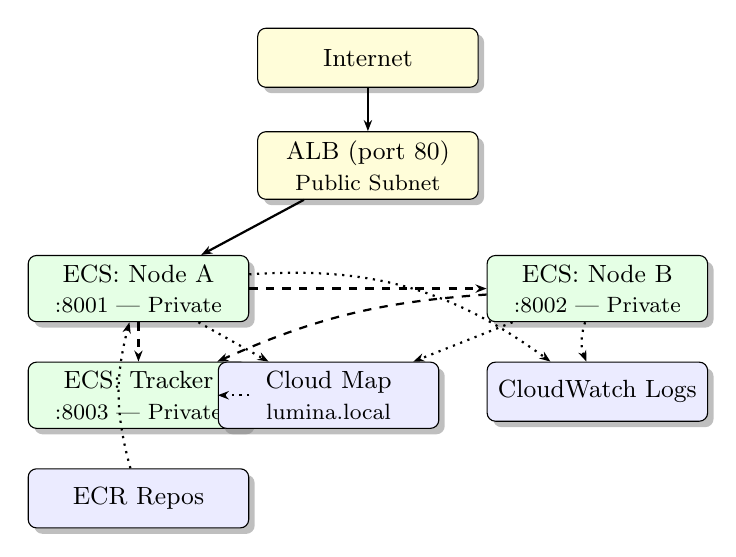
\begin{tikzpicture}[
  box/.style={rectangle, rounded corners=3pt, draw, minimum width=2.8cm,
              minimum height=0.75cm, align=center, font=\small, drop shadow},
  cloud/.style={box, fill=blue!8},
  ecs/.style={box, fill=green!10},
  pub/.style={box, fill=yellow!15},
  arrow/.style={-{Stealth[length=4pt]}, thick},
  node distance=0.55cm and 0.3cm
]

\node[pub] (inet) {Internet};
\node[pub, below=of inet] (alb) {ALB (port 80)\\\footnotesize Public Subnet};
\node[ecs, below left=0.7cm and 0.1cm of alb] (nodea)
  {ECS: Node A\\\footnotesize :8001 — Private};
\node[ecs, below=0.5cm of nodea] (tracker)
  {ECS: Tracker\\\footnotesize :8003 — Private};
\node[ecs, below right=0.7cm and 0.1cm of alb] (nodeb)
  {ECS: Node B\\\footnotesize :8002 — Private};
\node[cloud, below=0.5cm of tracker] (ecr) {ECR Repos};
\node[cloud, below=0.5cm of nodeb] (cw) {CloudWatch Logs};
\node[cloud, below right=0.5cm and -0.4cm of nodea] (cm)
  {Cloud Map\\\footnotesize lumina.local};

\draw[arrow] (inet) -- (alb);
\draw[arrow] (alb) -- (nodea);
\draw[arrow, dashed] (nodea) -- (nodeb);
\draw[arrow, dashed] (nodea) -- (tracker);
\draw[arrow, dashed] (nodeb) to[bend right=10] (tracker);
\draw[arrow, dotted] (nodea) -- (cm);
\draw[arrow, dotted] (nodeb) -- (cm);
\draw[arrow, dotted] (tracker) -- (cm);
\draw[arrow, dotted] (nodea) to[bend left=20] (cw);
\draw[arrow, dotted] (nodeb) to[bend right=20] (cw);
\draw[arrow, dotted] (ecr) to[bend left=15] (nodea);

\end{tikzpicture}
\caption{AWS Fargate production topology. ECS tasks run in private subnets.
The ALB handles public ingress. AWS Cloud Map provides service-to-service DNS
resolution. Solid arrows: data flow; dashed: control; dotted: infrastructure.}
\label{fig:fargate}
\end{figure}

% ─────────────────────────────────────────────────────────────────────────────
\section{Evaluation}

\subsection{Functional Validation}

The system was validated end-to-end using Qwen2.5-1.5B-Instruct (28
transformer layers, 1.5B parameters) across three nodes. Functional correctness
was confirmed by verifying that text generated via the three-node split pipeline
produces coherent completions. The autoregressive loop correctly terminates on
EOS token detection, and the rotary embedding buffers are correctly reconstructed
on CPU nodes via \texttt{\_ensure\_qwen2\_rotary\_buffers}.

\subsection{Latency Profile}

The tensor transport pipeline
(\texttt{torch.save} $\to$ base64 encode $\to$ HTTP POST $\to$ base64 decode
$\to$ \texttt{torch.load}) is executed twice per token (A$\to$B and B$\to$C).
Hidden state tensors for Qwen2.5-1.5B have shape $[1, L, 1536]$ (hidden
dimension 1536), roughly double that of GPT-2. Per-token inference time on
CPU-only instances is significantly higher, making network serialization a
smaller fraction of total latency.

With the three-node chain, total generation latency for $N$ tokens extends
the two-node formula to include the mid-node:

\begin{equation}
  T_{\text{total}} = N \cdot \left(T_A + T_{AB} + T_B + T_{BC} + T_C\right)
  \label{eq:latency}
\end{equation}

where $T_A$, $T_B$, $T_C$ are per-node inference times and $T_{AB}$,
$T_{BC}$ are the serialization + network costs for each hop.

\subsection{Dynamic Split Behavior}

With three nodes reporting equal VRAM (4.0\,GB each, the CPU fallback),
the Tracker assigns the 28 layers evenly: \texttt{split\_layer\_a}~$= 9$,
\texttt{split\_layer\_b}~$= 18$, giving a 9/9/10 distribution. The cloud
deployment uses a fixed 9/10/9 split via environment variables. The version
counter correctly detects boundary changes, allowing Node~A to refresh its
assignment without maintaining local state.

% ─────────────────────────────────────────────────────────────────────────────
\section{Enterprise Considerations}

\subsection{Microservices Architecture}

Lumina's four backend services map cleanly onto the microservices decomposition
pattern~\cite{newman2021microservices}. Each service owns a distinct
responsibility: Node~A orchestrates generation, Node~B relays mid-layer
computation, Node~C produces final tokens, and the Tracker manages
coordination. Services communicate exclusively via well-defined REST APIs with
Pydantic-validated request/response schemas, ensuring contract stability as
individual services evolve independently.

\subsection{Service Discovery Pattern}

Lumina implements a self-registration variant of the client-side service
discovery pattern~\cite{richardson2018patterns}. On startup, each node posts
its capabilities to the Tracker's \texttt{/register} endpoint. The Tracker
maintains the service registry in memory, with entries expiring after 30~s of
missed heartbeats. This is functionally equivalent to Consul's TTL check
mechanism or Kubernetes' readiness probe system, implemented without external
dependencies. The production Fargate deployment replaces runtime
self-registration with AWS Cloud Map, a managed service discovery solution
that integrates with ECS and Route~53.

\subsection{CAP Theorem Implications}

The Tracker service presents an interesting CAP theorem~\cite{brewer2012cap}
tradeoff. The in-memory registry prioritizes Availability and Partition
Tolerance (AP) over Consistency: if the Tracker becomes unreachable, Node~A
falls back to a static \texttt{split\_layer} value rather than blocking
generation. This is an intentional design choice---partial availability
(possibly suboptimal split assignment) is preferable to total unavailability.

The assignment version counter provides eventual consistency: nodes that have
been operating with a stale \texttt{split\_layer} will converge to the current
value on their next successful Tracker query. The system does not guarantee
that all active requests use the same split layer. A CP system would require
distributed consensus (e.g., Raft) for split assignment, introducing latency
unacceptable for interactive inference.

\subsection{Fault Tolerance}

Three fault tolerance mechanisms are implemented. First, the heartbeat timeout:
nodes that fail silently are detected within \texttt{heartbeat\_timeout\_sec}
(120~s in cloud deployments) and removed from the active assignment; the
background heartbeat thread in each node ensures liveness signals continue
even during idle periods. Second, the fallback split layer: when no active
tail node is registered, the Tracker returns the static
\texttt{fallback\_split\_layer}, preventing Node~A from blocking. Third,
Node~A's generate endpoint wraps the Node~B HTTP call in a try/except block,
returning HTTP~502 with a descriptive error rather than an unhandled exception.

\subsection{Infrastructure as Code}

All infrastructure is defined in Terraform HCL, enabling reproducible
deployments across environments. The EC2 configuration (\texttt{deploy-ec2/})
and Fargate configuration (\texttt{terraform/}) represent development and
production tiers respectively. Terraform state management via S3 and DynamoDB
locking supports team-based infrastructure management with conflict prevention.

\subsection{Observability}

Enterprise systems require observability across three pillars: metrics, logs,
and traces~\cite{sridharan2018observability}. Lumina implements a subset of
this stack appropriate for a Sprint~1 proof-of-concept. Structured JSON logs
are emitted by uvicorn to stdout and captured by Docker/CloudWatch. Per-request
traces record prompt, assigned nodes, status, and wall-clock duration. Health
endpoints provide pull-based liveness signals compatible with load balancer
health checks and Kubernetes readiness probes.

\subsection{Container Orchestration Tradeoffs}

The system supports two container orchestration approaches. Docker Compose (EC2
deployment) provides simplicity and low operational overhead suitable for
single-machine or small-cluster development. AWS ECS Fargate (production
deployment) provides managed task scheduling, auto-scaling, rolling deploys,
and integration with IAM, CloudWatch, and AWS Cloud Map. The tradeoff is
operational complexity versus capability: Fargate eliminates instance management
but introduces higher baseline costs (\$75/month vs.\ \$20/month for EC2 in
equivalent configuration).

% ─────────────────────────────────────────────────────────────────────────────
\section{Limitations \& Future Work}

\subsection{Current Limitations}

The following limitations are acknowledged in the current implementation:

\begin{itemize}
  \item HTTP/JSON transport for tensors introduces per-token serialization
        overhead not present in production split inference systems that use
        gRPC or NCCL.
  \item In-memory Tracker state is lost on restart. A production deployment
        requires persistent storage (Redis, DynamoDB) for the node registry
        and request trace history.
  \item The system supports exactly one head and one tail node. Horizontal
        scaling of either role requires a load balancing layer not yet
        implemented.
  \item Autoregressive generation returns the complete text after all tokens
        are generated. Streaming output via Server-Sent Events or WebSocket
        is not yet supported.
  \item CPU-only inference on \texttt{t3.small} is approximately 100$\times$
        slower than GPU-accelerated inference. The architecture is GPU-ready
        (CUDA device detection is implemented) but not validated on GPU
        hardware.
\end{itemize}

\subsection{Phase 2 Roadmap}

\begin{itemize}
  \item \textbf{gRPC transport:} Replace HTTP/JSON tensor transfer with gRPC
        and Protocol Buffers, eliminating base64 encoding overhead.
  \item \textbf{Streaming generation:} Server-Sent Events for progressive
        frontend token rendering.
  \item \textbf{Peer discovery:} mDNS/DHT-based node discovery to replace
        static Tracker registration.
  \item \textbf{Latency telemetry:} Per-step metrics
        ($T_{\text{encode}}$, $T_{\text{transfer}}$, $T_{\text{decode}}$,
        $T_{\text{tail}}$) to support data-driven split optimization.
  \item \textbf{N-node pipeline:} Extend the two-node model to arbitrary
        pipeline depth ($N$ nodes, $N-1$ split points).
  \item \textbf{Persistent Tracker:} Redis-backed node registry and request
        history.
\end{itemize}

% ─────────────────────────────────────────────────────────────────────────────
\section{Conclusion}

This paper presented Lumina, a distributed split inference system that
partitions a GPT-2 transformer across two compute nodes using a dynamic,
VRAM-proportional layer assignment algorithm. The system demonstrates that
enterprise distributed systems patterns---microservices decomposition, service
self-registration, heartbeat-based liveness, dynamic configuration, and
infrastructure as code---can be applied coherently to the domain of neural
network inference.

The Tracker's rebalancing algorithm enables the system to adapt split
assignments at runtime without service restarts, while the fallback mechanism
maintains availability in the face of node failure. The tensor transport
protocol, while not optimized for throughput, operates over standard HTTP and
requires no custom networking infrastructure, enabling deployment on commodity
AWS EC2 instances.

From a CAP theorem perspective, the system prioritizes Availability and
Partition Tolerance over Consistency in split assignment, accepting the
possibility of suboptimal layer partitioning during transient disagreement in
exchange for uninterrupted inference service. This tradeoff is appropriate for
interactive text generation workloads where latency consistency matters more
than perfect resource utilization.

Future work will address the primary performance limitation---HTTP-based tensor
transport---by introducing gRPC, and extend the pipeline to support $N$-node
parallelism and streaming output. The production Fargate deployment path
provides a clear upgrade trajectory from the current EC2 development
deployment.

% ─────────────────────────────────────────────────────────────────────────────
\appendix

\section{Technology Stack}

Table~\ref{tab:stack} lists the complete technology stack.

\begin{table}[htbp]
\centering
\caption{Lumina Technology Stack}
\label{tab:stack}
\renewcommand{\arraystretch}{1.15}
\begin{tabular}{llll}
\toprule
\textbf{Component}   & \textbf{Technology}       & \textbf{Version} & \textbf{Role} \\
\midrule
Backend runtime      & Python                    & 3.11             & Core language \\
Web framework        & FastAPI + uvicorn          & 0.116 / 0.35     & REST API      \\
ML framework         & PyTorch                   & 2.8.0            & Tensor ops    \\
Model library        & HuggingFace Transformers  & 4.54.1           & GPT-2 loader  \\
Data validation      & Pydantic v2               & 2.11.7           & Schemas       \\
Frontend             & React + Vite              & 19.2 / 8.0       & Dashboard     \\
Charting             & Recharts + ReactFlow      & 3.8 / 11.11      & Metrics UI    \\
HTTP client          & Axios                     & 1.15             & API calls     \\
Reverse proxy        & nginx                     & 1.28             & Static + proxy\\
Containerization     & Docker + Compose          & 25.0 / v2        & Isolation     \\
IaC                  & Terraform                 & 1.5              & Provisioning  \\
Cloud platform       & AWS EC2 / Fargate         & ---              & Compute       \\
Language model       & GPT-2                     & 117M params      & Inference     \\
\bottomrule
\end{tabular}
\end{table}

\section{REST API Reference}

Table~\ref{tab:api} summarizes all service endpoints.

\begin{table}[htbp]
\centering
\caption{Lumina REST API Endpoints}
\label{tab:api}
\renewcommand{\arraystretch}{1.15}
\begin{tabular}{lllp{2.8cm}}
\toprule
\textbf{Service} & \textbf{Method} & \textbf{Endpoint} & \textbf{Description} \\
\midrule
Node A   & GET  & \texttt{/health}             & Status, model, split \\
Node A   & POST & \texttt{/generate}           & Text generation \\
Node B   & GET  & \texttt{/health}             & Tail node status \\
Node B   & POST & \texttt{/forward\_tail}      & Run tail layers \\
Tracker  & POST & \texttt{/register}           & Node registration \\
Tracker  & POST & \texttt{/heartbeat}          & Liveness refresh \\
Tracker  & GET  & \texttt{/assignment}         & Current split \\
Tracker  & GET  & \texttt{/nodes/list}         & Node registry \\
Tracker  & GET  & \texttt{/assignments/current}& Layer ranges \\
Tracker  & GET  & \texttt{/requests/traces}    & Request history \\
\bottomrule
\end{tabular}
\end{table}

% ─────────────────────────────────────────────────────────────────────────────
\begin{thebibliography}{00}

\bibitem{radford2019gpt2}
A.~Radford, J.~Wu, R.~Child, D.~Luan, D.~Amodei, and I.~Sutskever,
``Language Models are Unsupervised Multitask Learners,''
\textit{OpenAI Blog}, vol.~1, no.~8, 2019.

\bibitem{kang2017neurosurgeon}
Y.~Kang, J.~Hauswald, C.~Gao, A.~Rovinski, T.~Mudge, J.~Mars, and L.~Tang,
``Neurosurgeon: Collaborative Intelligence Between the Cloud and Mobile Edge,''
in \textit{Proc. ACM Int. Conf. Architectural Support for Programming Languages
and Operating Systems (ASPLOS)}, 2017, pp.~615--629.

\bibitem{shoeybi2019megatron}
M.~Shoeybi, M.~Patwary, R.~Puri, P.~LeGresley, J.~Casper, and B.~Catanzaro,
``Megatron-LM: Training Multi-Billion Parameter Language Models Using Model
Parallelism,'' \textit{arXiv preprint arXiv:1909.08053}, 2019.

\bibitem{bai2020pipeswitch}
Z.~Bai, Z.~Li, Y.~Wang, and X.~Liu,
``PipeSwitch: Fast Pipelined Context Switching for Deep Learning Applications,''
in \textit{Proc. USENIX Symp. on Operating Systems Design and Implementation
(OSDI)}, 2020, pp.~499--514.

\bibitem{li2018jalad}
L.~Li, D.~Shen, and P.~Zhang,
``JALAD: Joint Accuracy and Latency-Aware Deep Structure Decoupling for
Edge-Cloud Inference,''
in \textit{Proc. IEEE Int. Conf. on Parallel and Distributed Systems
(ICPADS)}, 2018.

\bibitem{crankshaw2017clipper}
D.~Crankshaw, X.~Wang, G.~Zhou, M.~J.~Franklin, J.~E.~Gonzalez, and
I.~Stoica,
``Clipper: A Low-Latency Online Prediction Serving System,''
in \textit{Proc. USENIX Symp. on Networked Systems Design and Implementation
(NSDI)}, 2017, pp.~613--627.

\bibitem{kserve2023}
KServe Authors,
``KServe: Highly Scalable and Standards Based Model Inference Platform on
Kubernetes,'' GitHub Repository, 2023.
[Online]. Available: \url{https://github.com/kserve/kserve}

\bibitem{jeaugey2017nccl}
S.~Jeaugey,
``NCCL 2.0,''
in \textit{GPU Technology Conference (GTC)}, 2017.

\bibitem{newman2021microservices}
S.~Newman,
\textit{Building Microservices: Designing Fine-Grained Systems}, 2nd~ed.
Sebastopol, CA: O'Reilly Media, 2021.

\bibitem{richardson2018patterns}
C.~Richardson,
\textit{Microservices Patterns}.
Shelter Island, NY: Manning Publications, 2018.

\bibitem{brewer2012cap}
E.~Brewer,
``CAP Twelve Years Later: How the `Rules' Have Changed,''
\textit{IEEE Computer}, vol.~45, no.~2, pp.~23--29, Feb.~2012.

\bibitem{sridharan2018observability}
C.~Sridharan,
\textit{Distributed Systems Observability}.
Sebastopol, CA: O'Reilly Media, 2018.

\bibitem{qwen2025}
Qwen Team,
``Qwen2.5: A Party of Foundation Models,''
\textit{arXiv preprint arXiv:2412.15115}, 2025.

\end{thebibliography}

\end{document}
